\documentclass[10pt]{beamer}
\usepackage[utf8]{inputenc}
\usepackage{hyperref}
\hypersetup{colorlinks=true,linkbordercolor=blue,linkcolor=white,urlcolor=blue,pdfborderstyle={/S/U/W 1}}

\usepackage[scaled]{helvet}
\usepackage[T1]{fontenc}
\usetheme{Berkeley}
\beamertemplatenavigationsymbolsempty
\setbeamertemplate{headline}{}
\setbeamersize{sidebar width left=1.5cm}
\setbeamerfont{section in sidebar}{size=\fontsize{6}{6}\selectfont}
\setbeamerfont{title in sidebar}{size=\fontsize{6}{6}\selectfont}
\title{Geocoding with Photon}
\date{}

\begin{document}
\maketitle

\section{Topics}
\begin{frame}
\leftskip1em\textbf{Learn}
	\begin{itemize}
    \item what geocoding is
    \item how to use the Photon geocoding service
	\end{itemize}
\end{frame}

\section{1}
\begin{frame}
	\begin{center}
  		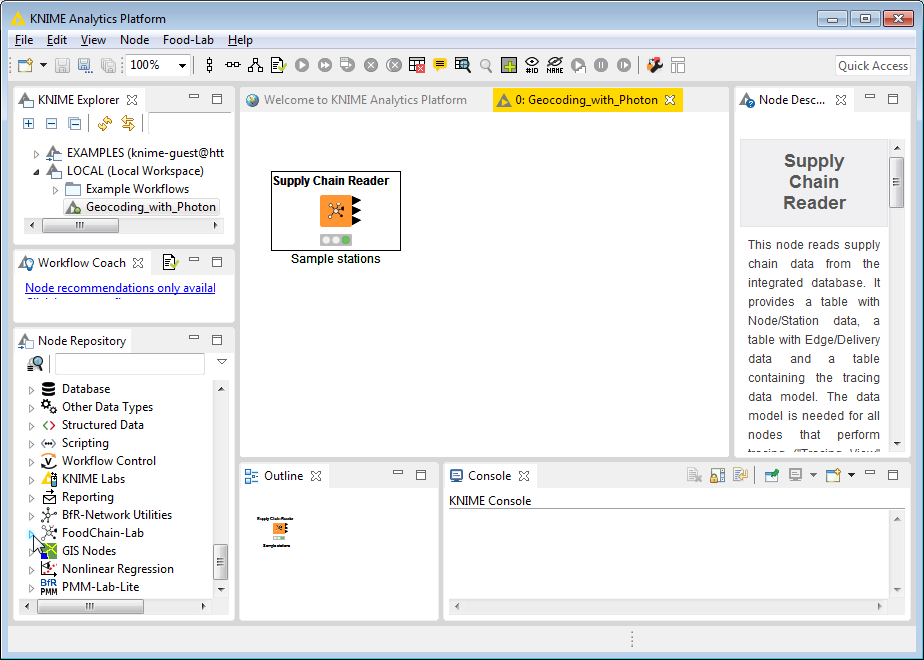
\includegraphics[height=0.6\textheight]{1.png}
	\end{center}
	\begin{itemize}
		\item Import the Geocoding workflow  \textcolor{blue}{\underline{\href{https://github.com/SiLeBAT/BfROpenLabResources/raw/master/GitHubPages/workflows/Geocoding\_with\_Photon.knwf}{``Geocoding\_with\_Photon.knwf''}}}.
		%\item In this tutorial we are using the Photon Geocoding service.
	\end{itemize}
\end{frame}

\section{2}
\begin{frame}
	\begin{center}
  		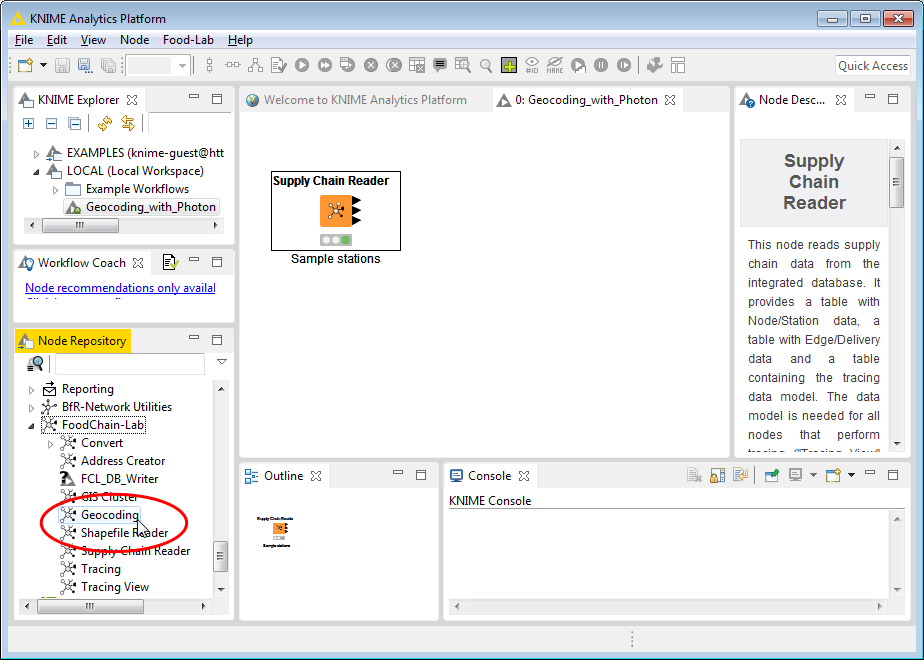
\includegraphics[height=0.6\textheight]{2.png}
	\end{center}
	\begin{itemize}
    \item To perform geocoding we need to add the \textbf{Geocoding} node. If the \textbf{Supply Chain Reader} is selected, double-click on the \textbf{Geocoding} node in the Node Repository.
    \item Another way to attach the \textbf{Geocoding} node to the \textbf{Supply Chain Reader} is to drag it from the Node Repository into the workflow editor and to connect the top outport of the \textbf{Supply Chain Reader} with the inport of the \textbf{Geocoding} node.
	\end{itemize}
\end{frame}

\section{3}
\begin{frame}
	\begin{center}
  		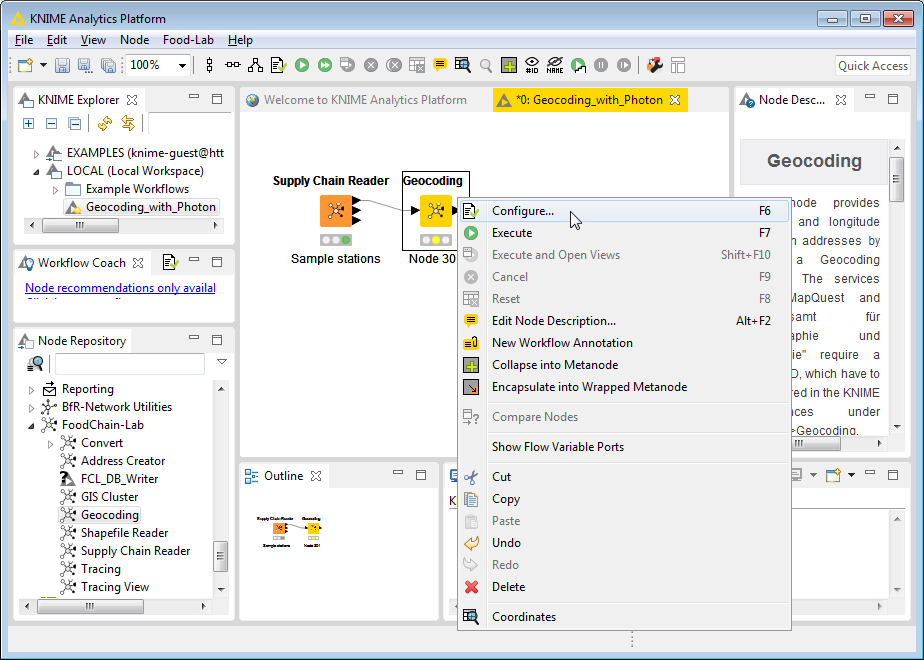
\includegraphics[height=0.6\textheight]{3.png}
	\end{center}
	\begin{itemize}
    \item The \textbf{Geocoding} node is connected to the \textbf{SupplyChainReader} and needs to be set up. Open its configuration by double clicking on it or by using its context menue (right click on the node, then choose ``configure'').
	\end{itemize}
\end{frame}

\section{4}
\begin{frame}
	\begin{center}
  		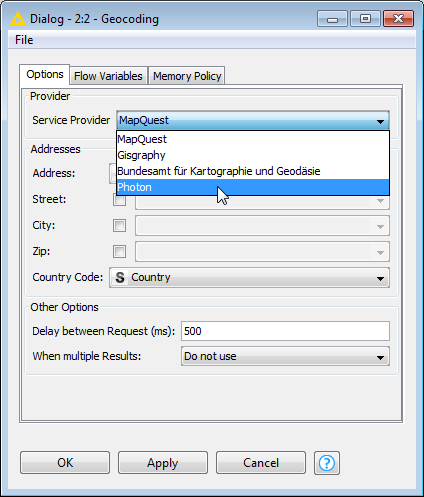
\includegraphics[height=0.6\textheight]{4.png}
	\end{center}
	\begin{itemize}
    \item Please choose the Service Provider ``Photon''.
	\end{itemize}
\end{frame}

\section{5}
\begin{frame}
	\begin{center}
  		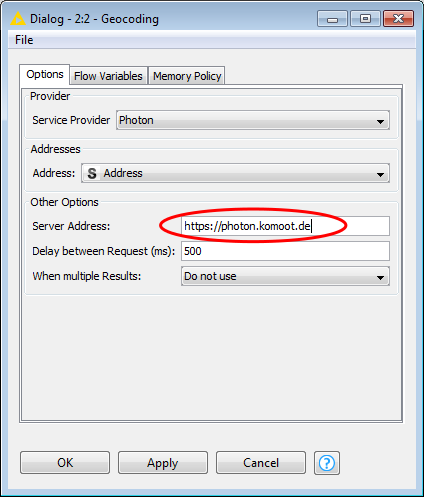
\includegraphics[height=0.6\textheight]{5.png}
	\end{center}
	\begin{itemize}
    \item The address is properly set, automatically.
		\item You need to set the server address. Please copy the URL  \url{http://photon.komoot.de} into the respective field. This is a publicly available service.
	\end{itemize}
\end{frame}

\section{6}
\begin{frame}
	\begin{center}
  		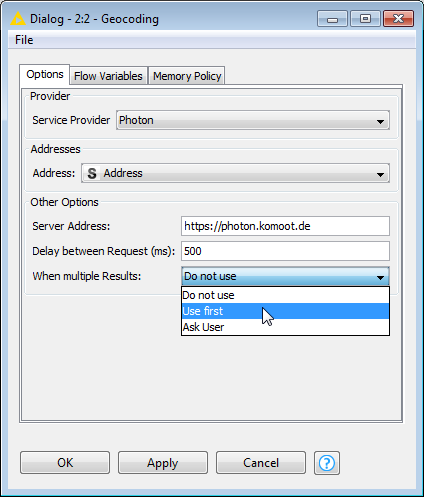
\includegraphics[height=0.5\textheight]{6.png}
	\end{center}
	\begin{itemize}
		\item For many requests geocoding services return multiple results, for example, if there are two streets with identical names. In the dropdown menu ``When muliple Results'' you can decide how to deal with this.
    \begin{itemize}
        \item[\textbullet] ``Do not use'': All multiple results will be discarded.
        \item[\textbullet] ``Use first'': The first entry of the multiple results list will be displayed for each address
		    \item[\textbullet] ``Ask User'': All multiple results will be displayed. The user needs to go through  all results and pick the favourite one menually. This is a lot of work for large data sets.
        \end{itemize}
  \end{itemize}
\end{frame}

\section{7}
\begin{frame}
	\begin{center}
  		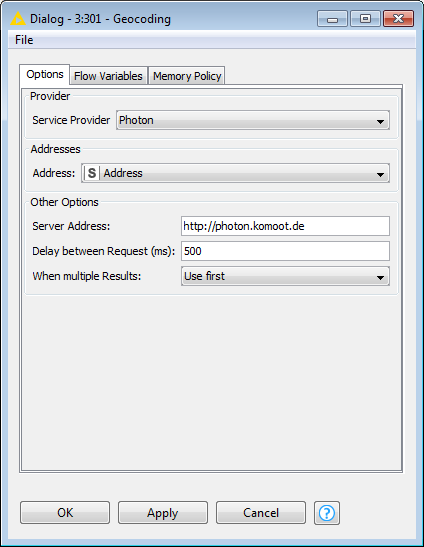
\includegraphics[height=0.5\textheight]{7.png}
	\end{center}
	\begin{itemize}
    \item In this tutorial select ``Use first'' and click ``OK''.
	\end{itemize}
\end{frame}

\section{8}
\begin{frame}
	\begin{center}
  		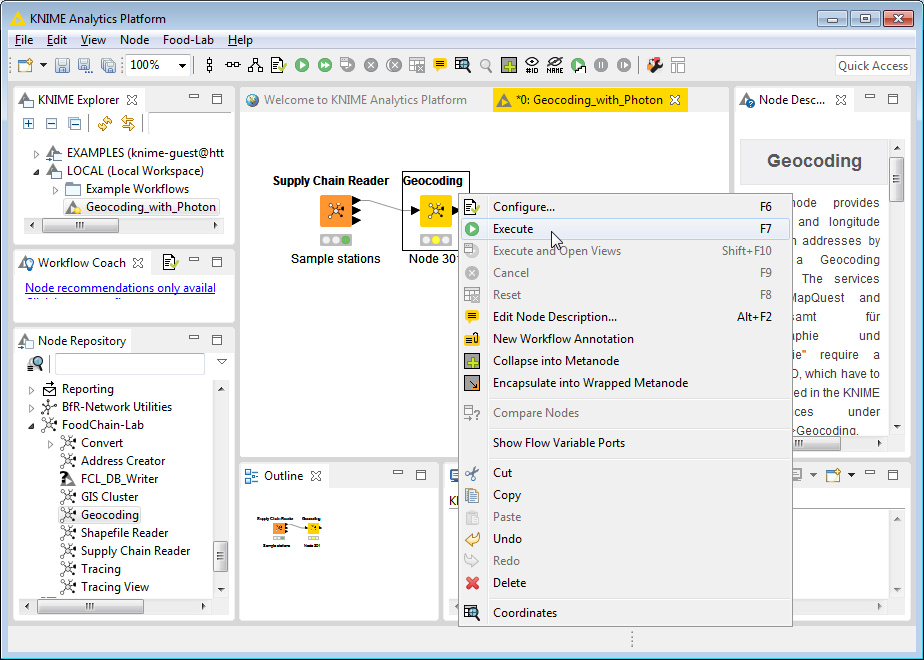
\includegraphics[height=0.6\textheight]{8.png}
	\end{center}
	\begin{itemize}
		\item Right click on the \textbf{Geocoding} node and select ``Execute''.
	\end{itemize}
\end{frame}

\section{9}
\begin{frame}
	\begin{center}
  		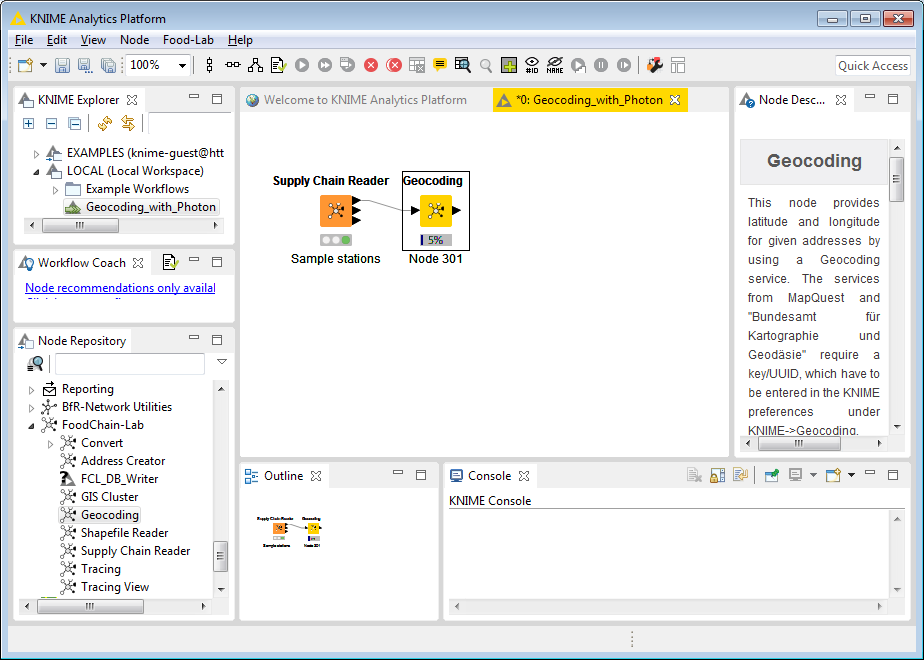
\includegraphics[height=0.6\textheight]{9.png}
	\end{center}
	\begin{itemize}
		\item The execution might take a while.
		\item The progress bar under the node shows the percentage of data which has been processed.
	\end{itemize}
\end{frame}

\section{10}
\begin{frame}
	\begin{center}
  		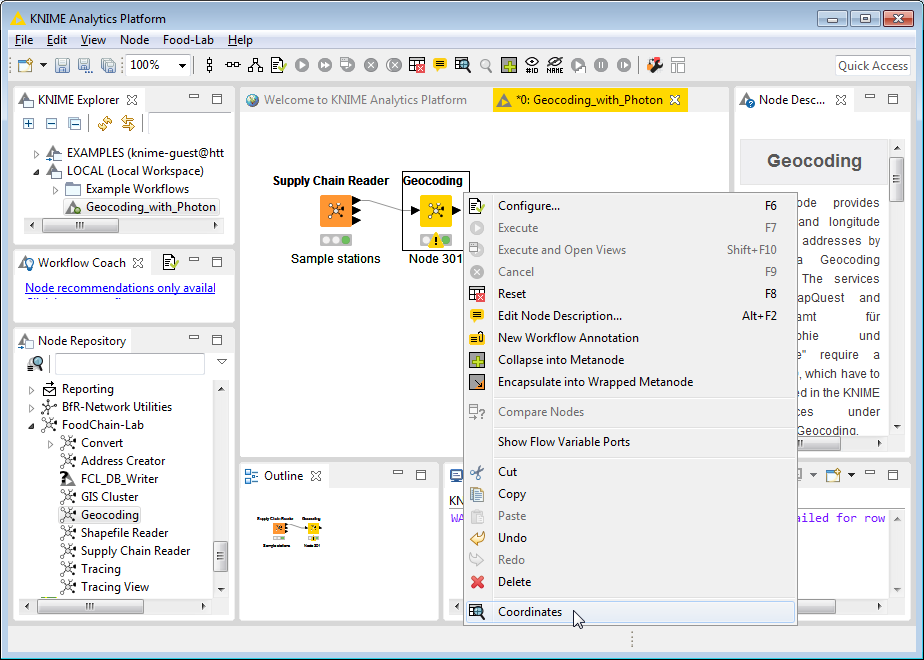
\includegraphics[height=0.6\textheight]{10.png}
	\end{center}
	\begin{itemize}
		\item When the execution is finished, we can look at the results.
		\item Right click on the \textbf{Geocoding} node and select ``Coordinates''.
	\end{itemize}
\end{frame}

\section{11}
\begin{frame}
	\begin{center}
  		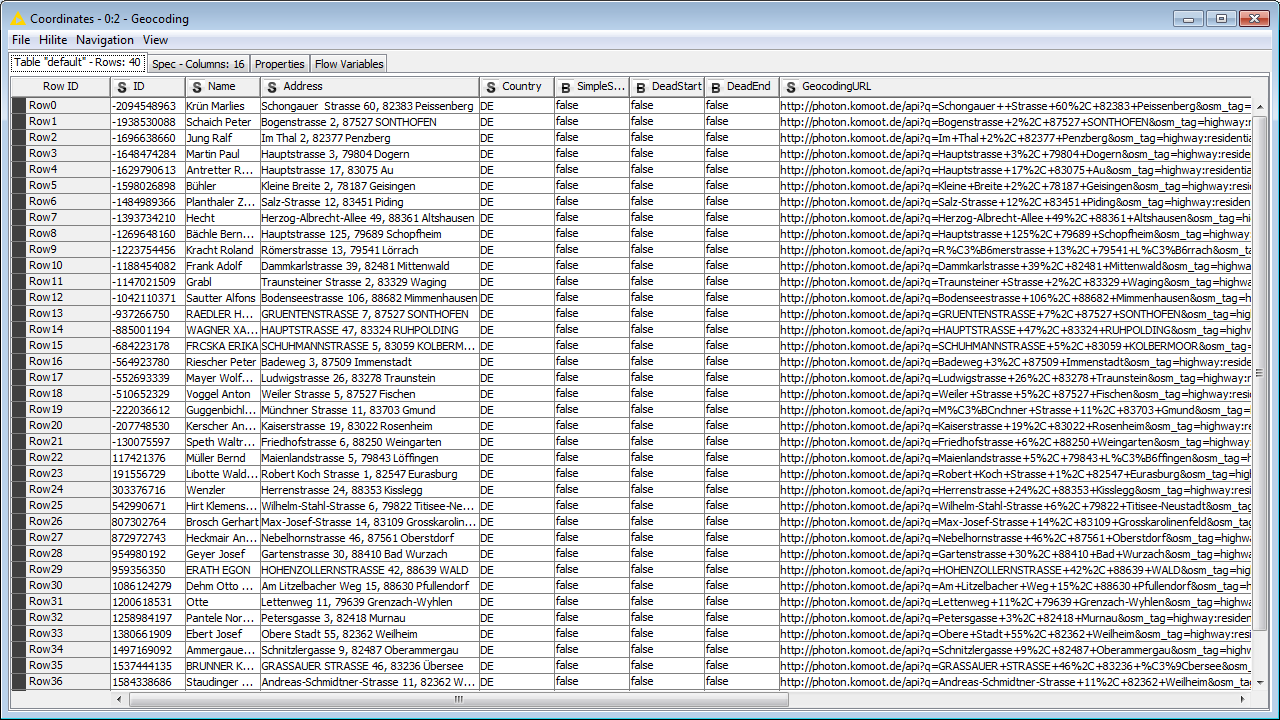
\includegraphics[height=0.6\textheight]{11.png}
	\end{center}
	\begin{itemize}
		\item In the dialog that pops up, you can look at the whole data table.
	\end{itemize}
\end{frame}

\section{12}
\begin{frame}
	\begin{center}
  		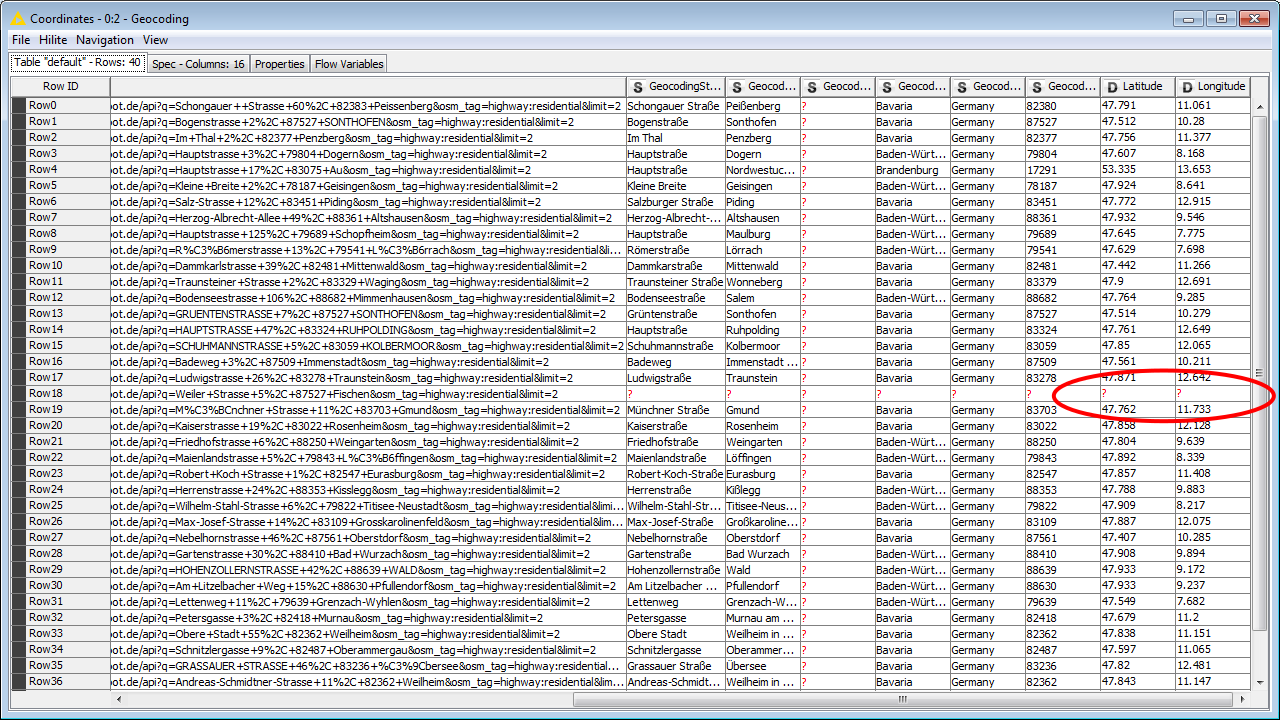
\includegraphics[height=0.6\textheight]{12.png}
	\end{center}
	\begin{itemize}
		\item Scroll to the right to look at the columns with latitude and longitude (the two rightmost columns).
		\item For 39 out of 40 addresses longitude and latitude could be found. One geocoding request was not successful.
	\end{itemize}
\end{frame}

\end{document}
